\section{Approach}
\label{sec:approach}
We first lay down some foundations for session-based recommendation, 
then present our base model which is a content-aware session-based model.
After that, we introduce the key ideas of neutral, positive, 
and negative feedback,
which are additional mechanisms that strengthen the base model. 
The high-level overview of our framework is illustrated in \figref{fig:arch}. 
%We introduce methods by which we utilize the temporal information and next zoom into each of the components to 
%present how our framework incorporates implicit positive and negative feedback.

\subsection{Session-based Recommendation Basics}
In a typical session-based setting, given the prefix sequence of the session, denoted as $S_u=(n_1, n_2,...,n_T)$, our goal is 
to predict $n_{T+1}$ article that the target user $u$ is most likely to click next. 
Following~\cite{liu2018stamp}, they use an $N\times d_n$ 
item embedding matrix, where $d_n$ is the embedding dimensionality, to provide article $n_i$'s embedding vector
as $\mathbf{x}_i$. Then methods like RNN~\cite{hidasi2018recurrent}, GNN~\cite{wu2019session,pan2020star}, 
or attention-based approaches~\cite{kang_self-attentive_2018,liu2018stamp} can be used to 
encode the session information into vector $\mathbf{x_s}$ from the sequence 
${(\mathbf{x}_1, \mathbf{x}_2, ..., \mathbf{x}_T)}$, which represents the user's history preferences.
Meanwhile, the same item embedding matrix can be also regarded as $N$ encoded candidates $[\mathbf{x}_1, \mathbf{x}_2,.., \mathbf{x}_N]$.
For $u$, the cosine similarity score $\hat{z_j}^u$ between the session representation and the article $j$ is calculated by the inner product of the session vector $\mathbf{x_s}$ and the candidate news article's vector:
\begin{equation}
    \label{eq:zj}
    \hat{z_j}^u = \mathbf{x}_j^T\mathbf{x_s}, j\in[1,N],
\end{equation}
\begin{equation}
    \label{eq:yy}
    \hat{\mathbf{y}}^u = softmax(\hat{\mathbf{z}}^u),
\end{equation}
$\hat{y_j}^u$ is normalized by softmax function in \eqnref{eq:yy} to be the probability of the article $j$ being clicked next in the session. 
The cross-entropy is usually used to compute loss:
\begin{equation}
    \label{eq:l1}
    \mathcal{L}_1 = - \frac{1}{|S|}\sum_{S_u \in S}\sum_{j=1}^N ( y_j^u \log(\hat{y_j}^u) + (1-y_j^u)\log(1-\hat{y_j}^u)),
\end{equation}
where $S$ is the whole training sessions, $y_j^u=1$ if the article $j$ is indeed the next-clicked articles $n_{T+1}$ in $S_u$ and $y_j^u=0$ otherwise.

\begin{figure*}[th]
    \centering
    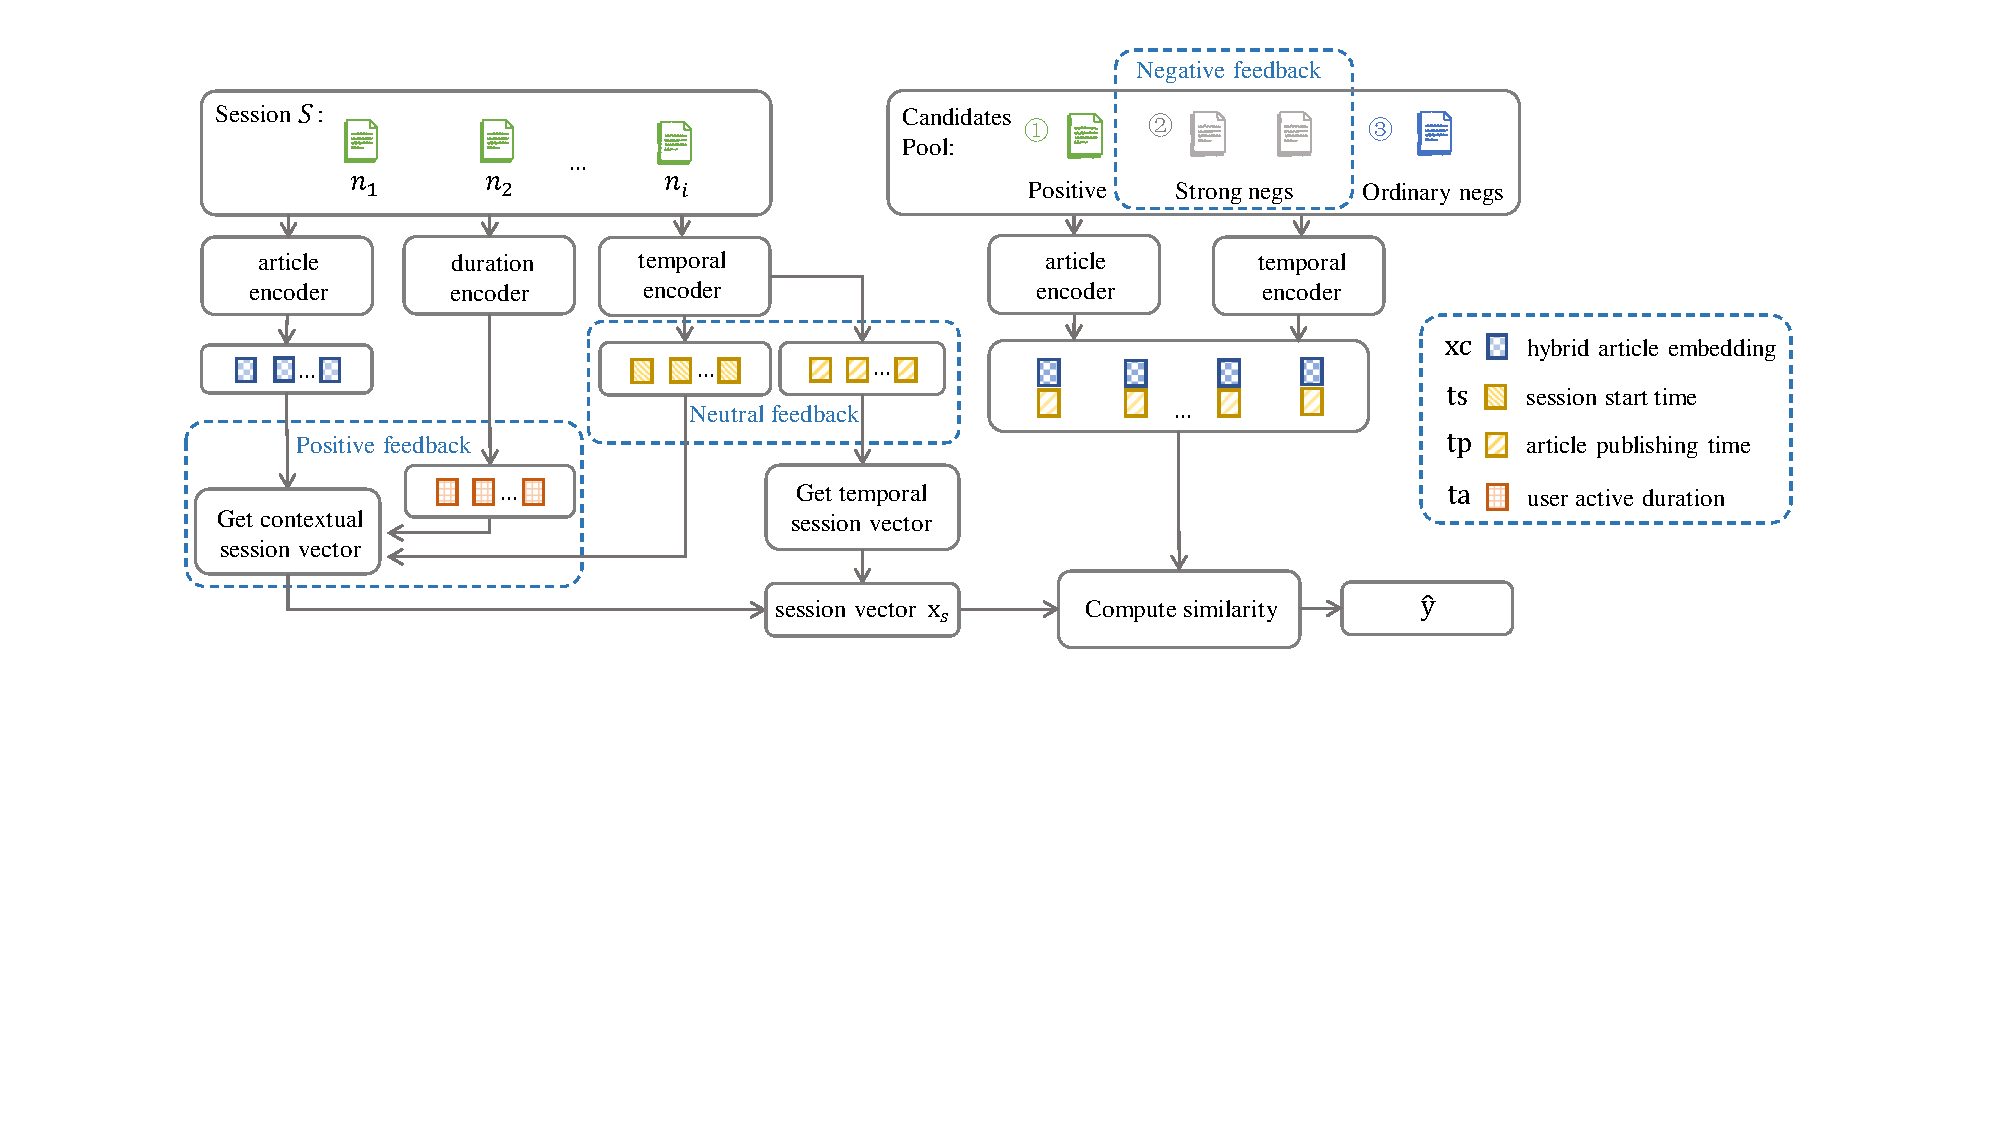
\includegraphics[width=0.95\textwidth]{fig/architecture.pdf}
    \caption{The architecture of our model. Squares in the figure represent
vectors, and their colors refer to the different encoders that produce them.}
    \label{fig:arch}
\end{figure*}

\subsection{Our Base Model: Content-aware Recommendation (CAR)}
\label{sec: base}
In order to recommend new and emerging articles,
our starting point is a basic content-aware recommendation model. 
To encode articles' content information, 
Some use pre-trained article content embeddings~\cite{gabriel2019contextual}, 
which is supervised trained based on the Word2Vec word embeddings in news titles and the metadata attributes of articles, such as categories.
Specifically, we get the $d_c$-dimensional vectors from Word2Vec to represent the 
topic-oriented content of articles. Once we get the content vector $\mathbf{c}_i$ of 
article $n_i$, we concatenate $\mathbf{c}_i$ and $\mathbf{x}_i$ to represent 
the article as $\mathbf{xc}_i$. 
To model the varying user preference to the articles in the same session, mainly following~\cite{liu2018stamp}, we adopt a simple attention network, using the weighted sum of the input sequence of vectors to encode the whole session.

We define $\alpha_i$, the attention weight of $i$-th articles $n_i$ in session $S_u$ as:
\begin{equation}
    \label{eq:alpha}
    \alpha_i = W_0 \times \sigma (W_1 \times \mathbf{xc}_i +  b_0),
\end{equation}
\begin{equation}
    \alpha_i^{\prime} = \frac{exp(\alpha_i)}{\sum_{i=1}^T exp(\alpha_i)},
\end{equation}
where $W_0\in \mathbb{R}^{1 \times d_n}, W_1 \in \mathbb{R}^{d_n\times (d_n+d_c)}$ 
are weighting parameters, $\mathbf{xc}_i$ is the vector representing the article, 
and $b_0\in \mathbb{R}^{d_n}$ is a bias. $\alpha_i^{\prime}$ is normalized by softmax function.

Finally, the contextual session vector $\mathbf{xc_s}$ of session $S_u$ is defined as the weighted sum:
\begin{equation}
    \label{eq:final_repre}
    \mathbf{xc_s} = \sum_{i=1}^{T} \alpha_i^{\prime} \mathbf{xc}_i.
\end{equation}

Noted that in order to obtain the sequential information of the input sequence, the attention mechanism extract $\mathbf{xc_s}$ utilizing the positional information by means of the positional encoding, which is the same as it is in Transformer architecture~\cite{vaswani2017attention}. In the end, we can optimize the loss function according to \eqnref{eq:zj}\textasciitilde\eqnref{eq:l1}; when computing $\mathcal{L}_1$, the $\mathbf{x}_j$ in \eqnref{eq:zj} should be replaced by $\mathbf{xc}_j$ and $\mathbf{x}_s$ is equal to $\mathbf{xc_s}$ in this base model.

\subsection{Modeling Time as Neutral Feedback}
\label{sec: temporal}
Active time that one user stays on one particular article is the duration time. For the different and continuous active time $t_i$, we design a duration encoder, which
bucketizes $t_i$ into a discrete variable~\cite{wu2020CPRS} by: 
\begin{equation}
   t_i^{\prime}=\lfloor log_2{t_i} \rfloor,
\end{equation}
and we map discrete $t_i^{\prime}$ into $m$ distinct categories, 
where each category shares the same embedding vector $\mathbf{ta}_i$.

Different from the duration time which reveals the positive implicit feedback 
from users, the date-time when a certain event happens carries physical 
meaning and also conveys the regular pattern behind the temporal information, 
hence we design a temporal encoder for this kind of temporal representation. We encode the publishing time of an article and the start time of a session. In order to extract periodic temporal change which is also known as seasonality, we feed 
the month, day of the month, day of the week, hour, minute $(s\in \mathbb{R}^{12}, d \in \mathbb{R}^{31}, w \in \mathbb{R}^7, h\in \mathbb{R}^{24}, m\in \mathbb{R}^{60})$ into a time embedding matrix $\mathbf{E_t}\in \mathbb{R}^{134 \times d_t}$ with $d_t$ dimension, and concatenate five parts as $\mathbf{t} \in \mathbb{R}^{5d_t}$ to build the whole temporal vector and to represent the date time. We next introduce how to utilize start time and publishing time, then we focus on modeling positive and negative implicit feedback which both derive from temporal information.

\subsubsection{Start time}
Users who start reading at a similar time are more likely to share the 
same reading behavior, which means that user interests are influenced by 
the start time. For example, some people tend to read financial news in 
the morning but instead read entertainment in the evening. 
We denote the click time from each click behavior of a session 
as $\mathbf{ts_i}\in \mathbb{R}^{2d_t}$ using the week and the hour $(w, h)$, which is enough to capture different user's daily routine. To model the different informativeness of the articles in $S_u$ for users' reading at different start reading time, we apply this information to compute personalized attention. We first transform the start time embedding vector $\mathbf{ts_i}$ into a preference query $\mathbf{q_i}$, which is similar to the ``query'' part in Transformer architecture:
\begin{equation}
    \mathbf{q_i} = ReLU(W_t \times \mathbf{ts}_i + b_t),
\end{equation}
where $W_t \in \mathbb{R}^{d_n \times 2d_t}$ is the projection parameter, $b_t \in \mathbb{R}^{d_n}$ is a bias.

Then we evaluate the importance of the interactions between preference query $\mathbf{q_i}$ and article representation $\mathbf{c}_i$ as attention $\alpha^{t}$:
\begin{equation}
    \alpha_i^{t} = \mathbf{c}_i \times tanh ( W_t^{\prime} \times \mathbf{q_i} + b_t^{\prime}),
\end{equation}
\begin{equation}
    \alpha_i^{t\prime} = \frac{exp(\alpha_i^{t})}{\sum_{j=1}^{|S_u|}exp(\alpha_j^{t})},
\end{equation}
where $W_t^{\prime} \in \mathbb{R}^{(d_c+d_n)\times d_n}$ and $b_t^{\prime} \in \mathbb{R}^{d_c+d_n}$ are weighting parameters. The contextual vector representation in \eqnref{eq:final_repre} is now modified to:
\begin{equation}
    \mathbf{xc_s} = \sum_{i=1}^{|S_u|} (\alpha_i^{\prime}+\alpha_i^{t\prime}) \mathbf{xc}_i.
\end{equation}

\subsubsection{Publish time}
Users' reading habits are reflected in the sequence of publishing time ${tp_1,...,tp_i}$ in $S_u$. We can make inferences whether the user tends to browse new articles or older ones from this. The publishing time of clicked articles is a relatively independent sequence thus we model it separately. Due to the high density of article publishing time, we construct publishing time embedding vector $\mathbf{tp}_i\in \mathbb{R}^{5d_t}$ using $(s, d, w, h, m)$. We obtain the session temporal representation vector $\mathbf{xt_s}$ by applying a similar attention mechanism in \secref{sec: base}. We add the content vector of each article to capture the attention relation between the article content and its publishing time. The attention weight with click-level content information involved is formulated as:
\begin{equation}
    \alpha_i^{tp} = W_0^{\prime} \times \sigma (W_1^{\prime} \times \mathbf{tp}_i + W_2^{\prime} \times \mathbf{c}_i + b_0^{\prime}),
\end{equation}
\begin{equation}
    \alpha_i^{tp\prime} = \frac{exp(\alpha_i^{tp})}{\sum_{j=1}^{|S_u|}exp(\alpha_j^{tp})},
\end{equation}
where $W_0^{\prime}\in \mathbb{R}^{1 \times d_n}, W_1^{\prime} \in \mathbb{R}^{(5d_t)\times d_n}, W_2^{\prime} \in \mathbb{R}^{d_c\times d_n}$ and $b_0^{\prime} \in \mathbb{R}^{1 \times d_n}$. The final temporal session representation is:
\begin{equation}
    \mathbf{xt_s} = \sum_{i=1}^{|S_u|} \alpha_i^{tp\prime} \mathbf{tp}_i.
\end{equation}

In the end, we concatenate $\mathbf{xt_s}$ and $\mathbf{xc_s}$ as the aggregated representation $\mathbf{x_s} \in \mathbb{R}^{d_n+d_c+5d_t} $ for the whole session. As for computing $\mathcal{L}_1$, the $\mathbf{x}_j$ in \eqnref{eq:zj} should be replaced by $\mathbf{xc}_j \oplus \mathbf{tp}_j$ ($\oplus$ stands for the concatenation operation).

\subsection{Modeling Positive Feedback}
\label{sec:positive feedback}
Our implicit positive feedback takes the form of the \textit{active time} interval that 
a user spent on each article after clicking on it. If the user spends a short time 
in an article, it's probably because the user is fooled by the title but actually does not like 
the article~\cite{lu_quality_2019}. Note that if the active time is not explicitly available, 
it can be estimated by the time interval between the user's two consecutive clicks. 

As illustrated in \secref{sec: temporal}, each degree of active time shares the same embedding vector $\mathbf{ta}_i$, representing to what extent the positive feedback is. We feed this vector into the attention computation as extra click-level 
feedback. Now, $\alpha_i$ in \eqnref{eq:alpha} is modified to:
\begin{equation}
    \alpha_i = W_0 \times \sigma (W_1 \times \mathbf{xc}_i + W_2 \times \mathbf{ta}_i + b_0),
\end{equation}
where $W_2 \in \mathbb{R}^{d_n \times d_t}$ is the projection parameter that map the active time embedding with $d_t$ dimension into another dimension space. The contextual session vector $\mathbf{xc_s}$ still follows
\eqnref{eq:final_repre} and final session vector $\mathbf{x_s}$ is combined with $\mathbf{xt_s}$ and $\mathbf{xc_s}$.

\subsection{Modeling Negative Feedback}
\label{sec:negative feedback}
The most straight-forward and widely adopted negative sampling strategy is the random sampling 
from a non-clicked set of items, or from a global buffer with the last $N$ 
clicks~\cite{gabriel2019contextual}. 
The major problem of randomly sampled items is that these items might be completely unrelated to 
the user, posing too little challenge for the model to learn. On the contrary, an informative item should be able to confuse the model whether it has discovered more complex hidden meaning of user interaction or not.

While reading news, a user scrolls up and down the news stream, 
and the articles that are exposed to the user collectively 
form an impression list $Imp_u$. We take unclicked articles in $Imp_u$ as more informative negative signals than other candidates~\cite{xie2020deep} and thus 
we should treat them differently when counting loss, which means we should penalize the similarity between $\mathbf{xc_s}$ and those strong negative samples more strictly. This idea is similar to utilizing grayscale data~\cite{lin2020world} and contrastive learning~\cite{saunshi2019theoretical}, where we both consider the different degrees of information carried from different items.

As we discussed before, since the impression list is not always explicitly available, 
we assume an article is more likely to be in $Imp_u$ if it was published nearby an article that has
been clicked by $u$. Specifically, we sort the candidate articles according to their publishing time, and keep the nearby articles with the window size 300 and sample items from this window.
We aim to minimize the cosine score between $\mathbf{xc_s}$ and the vector $\mathbf{xc}_j$ of negative sample $j$ when 
$j\in Ne_u$, where $Ne_u\subseteq Imp_u$ is the set of negative samples for session $S_u$, thus we add this constraint into the final loss: 

\begin{equation}
    \label{eq:loss}
    \begin{split}
        \mathcal{L}_2 = - \frac{1}{|S|} & \sum_{S_u \in S}\sum_{j=1}^N ( y_j^u \log(\hat{y_j}^u) + (1-y_j^u)\log(1-\hat{y_j}^u) \\
        & +  \lambda \mathbbm{1}(j \in Ne_u) \log(\sigma(1-\mathbf{xc}_j^T\mathbf{xc_s}))),
    \end{split}
\end{equation}
where $\mathbbm{1}(\cdot)$ returns 1 if the expression is true, $\lambda$ is 
the weighting parameter of loss from negative articles. We jointly optimize these two losses 
with Adam optimizer.
